% !TeX spellcheck = ru_RU
% !TEX root = vkr.tex

\section{Обзор}

В данном разделе представлен обзор существующих методов и технологий, связанных с процедурной генерацией интерьера. В частности, будут рассмотрены агентный и основанный на правилах подходы и некоторые особенности Unity-проекта.


\subsection{Существующие решения}

Исследователи в работе \enquote{Recent Advances in Procedural Generation of Buildings: From Diversity to Integration} \cite{kutzias2023recent} проанализировали существующие подходы к процедурной генерации интерьеров зданий. Около 67\% решений используют методы, \textit{основанные на правилах} (rule-based approach), около 23\% --- машинное обучение (machine learning) и около 6\% --- \textit{агентный подход} (agents approach). Наименьшее распространение получил способ \enquote{замены} (substitution approach), основанный на грамматиках. Системы, использующие машинное обучение, вопреки своей растущей популярности \cite{kutzias2023recent}, имеют существенный порог вхождения и требуют значительных временных трат \cite{kan2021automatic,balint2019generalized}. Таким образом, для решения поставленной задачи предпочтительнее использовать агентный или основанный на правилах подход (табл.\ref{tbl:comparison}).

\begin{table}[b]
\begin{center}
    \caption{Сравнение методов процедурной генерации интерьеров}
    \label{tbl:comparison}
    \rowcolors{2}{black!2}{black!10}
    \scalebox{0.7}{
    \begin{tabular}{|c|c|c|c|c|}
    \hline
    Критерий & Rule-based & Machine learning & Agents & Substitution \\
    \hline
    \hline
    Сложные иерархические  паттерны  & \ding{51} & \ding{51} & \ding{55} & \ding{51} \\
    Расстановка в реальном времени  & \ding{51} & \ding{51} & \ding{51} & \ding{51} \\
    Простота реализации & \ding{51} & \ding{55} & \ding{51} & \ding{55} \\
    Место по кол-ву научных публикаций & 1 & 2 & 3 & 4 \\
    \hline
    \end{tabular}
    }
\end{center}
\end{table}

\subsubsection{Агентный подход}

Исследователи под руководством Germer \cite{germer2009procedural} представили систему расстановки мебели, работающую в режиме реального времени. В ней каждый предмет интерьера является автономным агентом и обладает способностью к перемещению и оценке собственного положения. По словам авторов, у системы имеются некоторые недостатки. Например, нельзя явно указать телевизору на необходимость размещения на стене прямо напротив дивана или задать другие сложные иерархические зависимости. А в условиях быстрого перемещения пользователя система не успевает заполнить достаточное количество комнат.

\begin{figure}
  \centering
  \begin{minipage}{0.45\textwidth}
    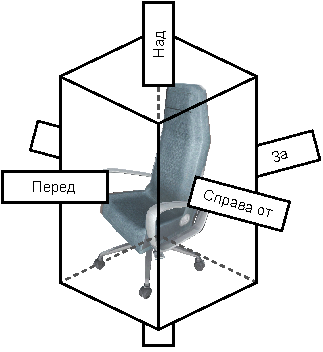
\includegraphics[width=0.8\textwidth]{matmex-diploma-template-master/figures/collider.pdf}
    \caption{Ограничительная рамка вокруг стула разделяет пространство вокруг на шесть зон}
    \label{fig:collider}
  \end{minipage}
  \hfill
  \begin{minipage}{0.45\textwidth}
    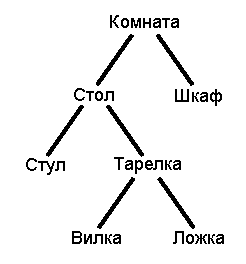
\includegraphics[width=0.8\textwidth]{matmex-diploma-template-master/figures/child_parent_relationship.pdf}
    \caption{Иерархическое представление комнаты}
    \label{fig:room_relationship}
  \end{minipage}
\end{figure}

Также в работе уделяется внимание представлению генерируемых объектов в виде упрощенных фигур. Исследователи пришли к выводу, что прямоугольный параллелепипед является хорошим приближением для многих объектов мебели. В таком представлении каждый предмет имеет ровно шесть граней, что сводит всевозможные случаи расстановки объектов к простым \enquote{перед}, \enquote{за}, \enquote{справа от} и т.~д (рис. \ref{fig:collider}). Наряду с этим авторы рассматривают концепцию детско-родительских отношений между предметами мебели, на вершине которой располагается вся декорируемая комната (рис. \ref{fig:room_relationship}).

\subsubsection{Основанный на правилах подход}

Идеи представления объектов, упомянутые выше, прослеживаются в работе \cite{lidberg2020hierarchical}. Предлагаемую в ней систему можно разделить на две составляющее: входные данные для генерации и сам алгоритм расстановки.

Входные данные определяются таблицей, содержащей сведения о всевозможных предметах мебели и их характеристиках.
Каждой строке соответствуют правила размещения объекта, вероятность его появления в различных пространствах, список предметов, которые он способен породить, и информация о том, является ли объект листовым, т.~e существующем исключительно по запросу родительского объекта. В свою очередь, алгоритм выражается в последовательности из шести шагов: инициализация генератора, выбор объекта, размещение и поиск свободного пространства, размещение листовых предметов и рекурсивный переход к заполнению дочерних пространств. В случае неудачи на некоторых шагах алгоритм способен вернуться на несколько итераций назад и повторить действия, пока положительный ответ не будет получен. Такое поведение может привести к неразрешимым сценариям, при которых время работы алгоритма окажется существенным, но в конечном итоге результат обещает быть более предсказуемым. 

После проведения независимого оценивания стало понятно --- система более чем способна генерировать реалистичные интерьеры. Участникам опроса до конца не сообщалось о целях его проведения, и многие из них были уверены, что помогают человеку-дизайнеру подобрать лучшее интерьерное решение.

\subsection{Особенности Unity-проекта}

Как было упомянуто раннее, Time Reactor --- это игра, созданная с использованием игрового движка Unity. До этого времени этажи заполнялись уже готовыми экземплярами комнат --- по одному на каждый тип помещения. Задача процедурной генерации интерьера, в свою очередь, заключалась именно в заполнении пустых версий этих комнат без изменения их размера и пропорций. В ином случае следует говорить о \textit{процедурно генерируемом экстерьере}.

Специфика Unity Engine позволяет использовать в игровых скриптах язык семейства .NET --- C\#. Это делает возможным интеграцию в проект библиотек на другом языке .NET --- F\#. Использование F\# для разработки библиотеки процедурной генераци обеспечило высокий уровень читабельности и чистоты кода благодаря функциональной парадигме языка. В том числе, неизменяемые данные поспособствовали более надежному и предсказуемому поведению алгоритмов, что особенно важно при создании систем генерации. Кроме того, такой подход позволил отделить генератор от игры и открыл новые перспективы для использования алгоритма в других проектах.  

\subsection{Генератор псевдослучайных чисел}

Генератор псевдослучайных чисел решает проблему сохранения интерьера комнаты при ее повторном посещении. При инициализации на вход генератору поступает число, называемое \textit{random seed} или просто \textit{seed}. Одинаковые входные значения seed гарантируют одну и ту же последовательность чисел, выдаваемых генератором, при каждом запуске программы. 

В качестве псевдослучайного генератора в проекте используется экземпляр класса \texttt{Random} из пространства имен \texttt{System}. Входными данными для него служит номер этажа --- уникальное число, характеризующее каждую из комнат.
 